\documentclass[a4paper, 12pt, titlepage, oneside]{article}

\usepackage[francais]{babel}
\usepackage{fancyhdr}
\usepackage{graphicx}
\usepackage{amsmath}
\usepackage[backend=biber]{biblatex}
\usepackage{subcaption}

\graphicspath{ {images/}}
\addbibresource{Biblio.bib}

\author{Martin Olivier, Fabien Goglio}
\title{Rapport InSite}

\pagestyle{fancy}

%Put the chapter and section header in lowercase
%\renewcommand{\chaptername}[1]{%
%	\markboth{#1}{}}

\renewcommand{\sectionmark}[1]{%
	\markright{\thesection\ #1}}

%delete the current header
\fancyhf{}

\fancyhead[LE, RO]{\bfseries\thepage}
\fancyhead[LO]{\bfseries\textit\rightmark}
%\fancyhead[RE]{\bfseries\textit}
\fancyhead[RE]{WAT}
\renewcommand{\footrulewidth}{0.5pt} %space for the rule
\fancypagestyle{plain}{\fancyhead{}, %get rid of header on plain pages
	\renewcommand{\headrulewidth}{0pt} % and the line
}


\begin{document}
\maketitle

\pagenumbering{roman}
\newpage
	\tableofcontents
\newpage
\cleardoublepage
\pagenumbering{arabic}
\section{Remerciement}
	Nous tenons a remercier \[...\]
	\newpage
\section{Introduction}
	\newpage
\section{Presentation}
	\subsection{Description}
		InSite analyse et detecte des objets archeologiques dans des releves geomagnetiques, en utilisant des techniques novatrices dans le domaine de
		la Computer Vision, ainsi que de l'apprentissage automatique.
	\subsection{Objectifs}
	Nous cherchons a:
	\begin{itemize}
		\item Manger 
		\item Boire
	\end{itemize}

	\newpage

\section{Cadrage}
	\subsection{Budget}
	\subsection{Dates clefs}
	\subsection{Organisation}
	\subsubsection{Demarche}
	\subsection{Planning}

	\newpage

\section{Demarche Initiale}
	\subsection{Detections d'objets}
	Nous avons decide de debuter nos recherches de detections de formes par des solutions simples, avec l'attente qu'elle nous donnent des resultats de bonne qualite. L'attrait de ces 
	methodes etaient principalement qu'elles ne requiert pas de quantite de donnees importante, et qu'elles etaient a notre porte d'un point de vue academique. Nous avons donc approche
	le probleme de deux facons differentes:
	\begin{itemize}
		\item Filtrage
		\item Algorithmes de detections de bords.
	\end{itemize}
	\subsubsection{Filtrage}
	{TODO: REMPLIR}
	
	\subsubsection{Algorithmes de detections de bords}
	Nous avons debute par l'utilisation de l'operateur de Sobel. Cet technique produit des images en noir et blanc ou les bords ont une valeur de blanc eleve. Un bord est defini comme un endroit de l'image ou la magnitude de son gradient est eleve. Son fonctionnement est decrit en plus de details ci-dessous: 
		\paragraph{\textbf{Recherche du gradient d'intensite de l'image}}
				On applique un kernel de Sobel: il s'agit simplement de deux matrices 3x3 permettant de calculer la derive premiere verticale et horizontale par convolution. Ces deux matrices sont:
				\\ \[G_x = \begin{bmatrix}  +1  & 0 & -1 \\ +2 & 0 & -2  \\ +1 &  0 & -1\end{bmatrix} 
					 G_y = \begin{bmatrix} +1 & +2 & +1  \\  0 & 0 &  0  \\ -1 & -2 & -1\end{bmatrix}\]
	A chaque point de l'image on determine la magnitude de ce gradient par la formule
					\[\nabla(G) = \sqrt{G_x^2 + G_y^2}\]
	\paragraph{\textbf{Creation d'une image des bords}}
	Une fois cet operation realise, il nous suffit d'associer la valeur du gradient a une valeur de gris. Une grande magnitude du gradient, indiquant que le pixel orignal appartenait a un bord donnera un pixel blanc, tandis qu'une faible intensite donnera un pixel noir.
	Sur des images "propres" on obtient ce genre de resultats: \\
	\begin{figure}[!h]
		\centering
		\begin{subfigure}[b]{0.4\linewidth}
			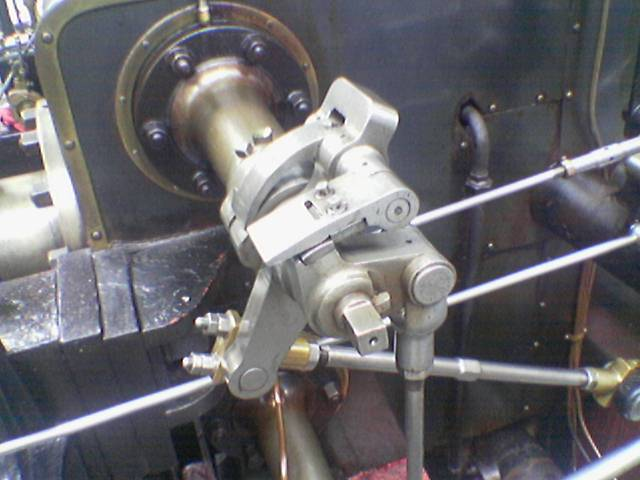
\includegraphics[width=\linewidth]{ValveOriginal.png}
			\caption{Image originelle}
		\end{subfigure}
		\begin{subfigure}[b]{0.4\linewidth}
			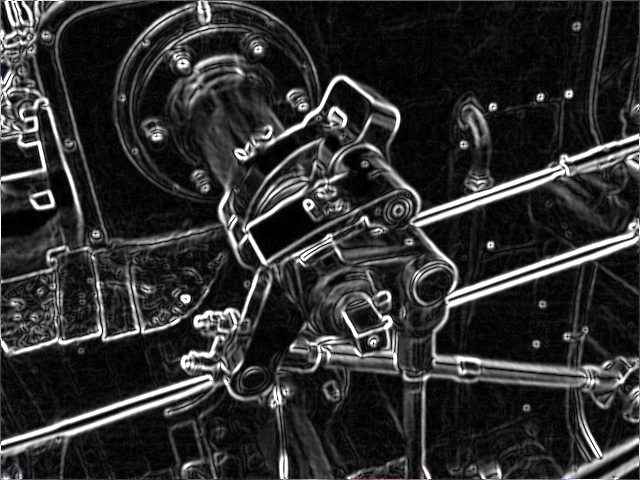
\includegraphics[width=\linewidth]{ValveSobel.png}
			\caption{Image traite avec Sobel}
		\end{subfigure}
		\label{fig:SobelGood}
	\end{figure}
	On observe que les details de l'image disparaissent, et que les bords, c'est a dire les endroits ou la magnitude du gradient de l'image sont important sont visible par des nuances de gris.\\
	Lorsque l'on applique l'operateur Sobel sur nos images, nous obtenons, dans les meilleurs des cas, ces resultats:
	\begin{figure}[!h]
		\centering
		\begin{subfigure}[b]{0.4\linewidth}
			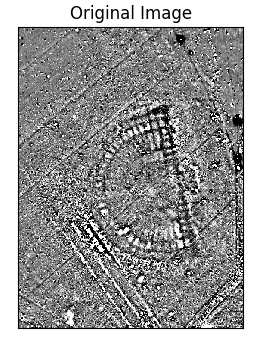
\includegraphics[width=\linewidth]{Sobel1b.png}
			\caption{Image originelle}
		\end{subfigure}
		\begin{subfigure}[b]{0.4\linewidth}
			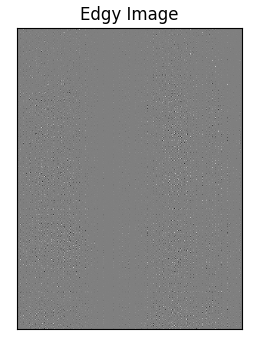
\includegraphics[width=\linewidth]{Sobel1a.png}
			\caption{Image traite avec Sobel}
		\end{subfigure}
		\label{fig:OurSobel}
	\end{figure}

	Sur nos images, les resultats obtenus ne sont pas tres pertinant. Le bruit est trop prevalent, et les bords des objets que nous cherchons a detecter sont trop faibles pour que l'operateur de Sobel puisse donne des resultats interessant.
	
	Malgres des resultats peu encouragant avec Sobel, nous avons decide d'utiliser un autre algorithme, celui de Canny. L'algorithme de Canny reprend les matrices de Sobel, et applique quelques operations supplementaire pour obtenir des bords plus precis. Les details de l'algorithme sont decrit ci-dessous:
	\begin{enumerate}
		\item \textbf{Reduction du bruit:}\\
			\indent On applique un filtre Gaussien 5x5 pour reduire le bruit present dans l'image
		\item \textbf{Recherche du gradient d'intensite de l'image:}\\  
		 	\indent On applique ensuite un kernel de Sobel sur l'image "lisse" dans les directions verticales et horizontales afin d'obtenir les derives premieres dans
		la direction verticale $G_x$ et horizontales $G_y$. Ce procede est identique a celui decrit plus haut.

		\item \textbf{Suppression des non maximums locaux}\\
			\indent Une fois les gradients obtenus, on analyse tout les pixels de l'image, et on determine si le pixel est un maximum local dans la
			direction du gradient. \\
			Si oui, c'est un bord et sa valeur est garde pour la prochaine etape, sinon, elle est mise a 0. On obtient une image binaire, avec que des bords

		\item \textbf{Seuil d'Hysterisis} \\
			\indent On utilise deux seuils, $minVal$ et $maxVal$. Tout les bords ayant une intensite de gradient superieur a $maxVal$ est forcement un
			bord, ceux en dessous de $minVal$ sont forcement des non-bords, et sont donc abandonne. Les bords qui sont entre ces deux seuil sont classe
			"bords" ou "non-bords" selon leur connectivite. Si ils sont connecte a des pixels qui sont des forcement des bords, alors ce sont des bords,
			sinon, ils sont aussi abandonne.\\
		
	\end{enumerate}
	Cet algorithme etant deja disponible dans la librairie d'analyse de d'image PythonCV2, nous n'avons pas eu a l'implementer, et nous avons beneficie de quelques optimisations rendant l'execution plus rapide.
	Avec une image "propre", on obtient ce genre d'image:\\
	\begin{figure}[!h]i %%NE PAS OUBLIER DE LINK L'AUTEUR : By Simpsons contributor, CC BY-SA 3.0, https://commons.wikimedia.org/w/index.php?curid=8904364
		\centering
		\begin{subfigure}[b]{0.4\linewidth}
			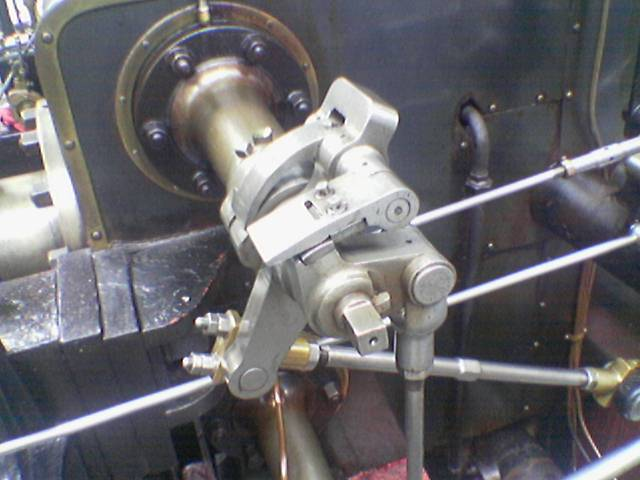
\includegraphics[width=\linewidth]{ValveOriginal.png}
			\caption{Image originelle}
		\end{subfigure}
		\begin{subfigure}[b]{0.4\linewidth}
			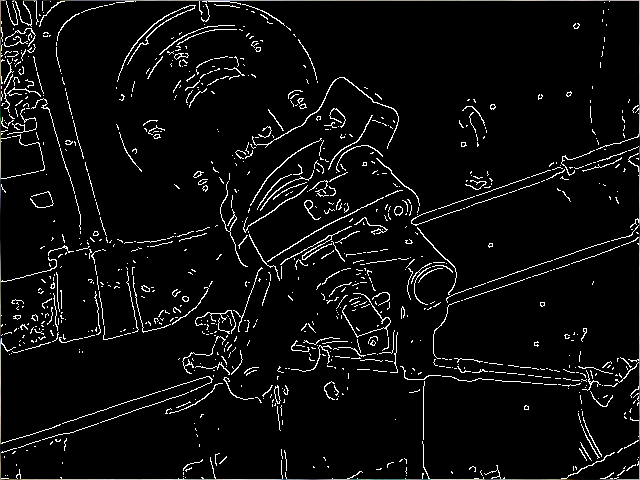
\includegraphics[width=\linewidth]{ValveCanny.png}
			\caption{Image traite avec Canny}
		\end{subfigure}
		\label{fig:cannyGood}
	\end{figure}
	On observe que les bords sont bien plus defini, et propre par rapport a ceux obtenu avec l'operateur Sobel. Mieux, les bords "majeurs", sont preserve, alors que les bords "mineurs" disparaissent. Cela est du aux deux dernieres etapes de l'algorithme de Canny.
			Lorsque l'on applique Canny a nos images, nous obtenons ceci:
	\begin{figure}[!h]
		\centering
		\begin{subfigure}[b]{0.4\linewidth}
			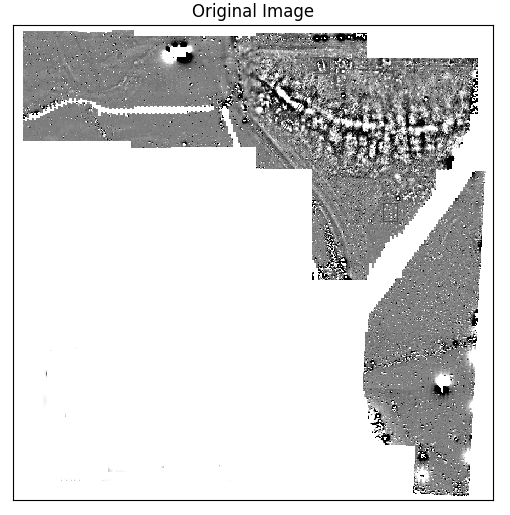
\includegraphics[width=\linewidth]{Canny1a.png}
			\caption{Image originelle}
		\end{subfigure}
		\begin{subfigure}[b]{0.4\linewidth}
			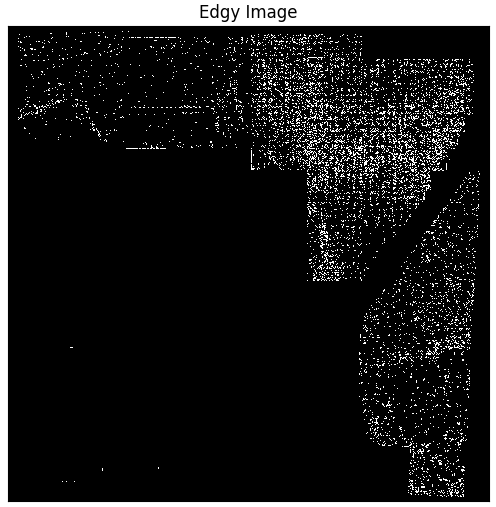
\includegraphics[width=\linewidth]{Canny1b.png}
			\caption{Image traite avec Canny}
		\end{subfigure}
		\label{fig:OurCanny}
	\end{figure}
	
	Meme si il y a une amelioration certaine par rapport a Sobel, l'algorithme ne parvient toujours pas a trouver les contours des objets d'interet, encore une fois a cause du a la grande quantite de bruit que l'on trouve dans l'image. Cependant  on observe une densite de points plus eleve aux niveau des endroits d'interets, comme ici, et une densite faible dans les zones ou on ne trouve ni objets ni bruit.
	
	TODO: AJOUTER PHOTO DETAILS 
	

	
	\subsubsection{Problemes rencontres}
	De toute evidence, nous avions atteint un obstacle: le bruit. Celui ci etait present sur toutes les images, au point d'empecher toute tentative d'analyse classique de signal. La magnetometrie est tres sensible aux objets metalliques, et dans la region ou ont ete fait les releves, de nombreux objets metalliques contemporrains sont present dans le terrain, notamment a cause des combats de la 2\textsuperscript{eme} guerre mondiale, mais aussi a cause des labours, et du dechets metallique produit par l'occupation humaines de ces terrains.\\
	Une analyse classique ne suffisait donc pas, et le developpement de methodes de filtrage et de detection de bords etant capable de traiter des images aussi bruite est hors de notre porte. Notre attention devait donc se porter sur la resolution d'un probleme, annexe a celui qui nous interessait, mais dont les techniques develope par sa resolution pouvait nous aider dans notre objectifs principal.
	TODO: A REMPLIR
	
\newpage
\section{Developement d'une nouvelle methodologie}
	\subsection{Detections de bruits par reseaux neuronal}
	Comme dit plus haut, les techniques classiques utilise dans l'analyse d'image sont innaplicables dans notre cas, du notament au haut niveau de bruit present dans les images a traites. Cependant, il est evidents que ce bruit n'est pas identique aux objets que nous cherchons, car sinon, les archeologues ne pourrait pas analyser ces images. Pour mieux diriger nos recherches nous avons choisi de detecter non pas un objets archeologique, mais un type de bruit tres prevalent dans ces images: un dipole. Les differences entre ce bruit et le reste de l'image etant trop subtils pour y etablir un ensemble de regles predefinie, nous avons decide d'utiliser des reseaux de convolution, qui sont un type de reseaux neuronaux, tres adaptes a l'analyse d'image pour detecter automatiquement le bruit, dans l'espoir de non seulement nettoyer le bruit, avec par exemple un flou Gaussien, mais egalement de detecter les objets archeologiques.
	\subsubsection{Caracterisation}
	Les dipoles proviennent des objets metalliques contemporains, et se caracterisent par un pole positif tres fort au niveau de l'objet, suivi d'un halo circulaire negatif, dont le diametre est approximativement 2 fois celui de l'objet.
	%RAJOUTER IMAGE DIPOLE REEL
	%RAJOUTER PLOT3D DIPOLE
	\subsubsection{Explication de l'approche}
	Les reseaux de convolution sont une innovation recente dans le champs de l'apprentissage automatique. Le premier exemple d'un reseau de convolution moderne provient de Yann Le Cun \cite{lecun-01a} en 1998. En 2012, les reseaux de convolution reapparaitront avec AlexNet \cite{NIPS2012_4824}, et restent aujourd'hui sur le devant de la scene de l'apprentissage automatique. 
	Les reseaux de convolutions, que nous appellerons CNNs (Convolutionnal Neural Network) se composent de 2 parties
	%EXPLICATION CNNS
	\subsubsection{Problemes initiaux}
	\subsubsection{Solutions}
	\textbf{Generation d'exemple}:\\
	Classifier a la main tout les exemples necessaires a l'entrainement du reseau etait une tache surhumaine. Par soucis d'efficacite, nous avons decide de construire nous meme
	nos exemples, et des les utiliser en combination avec des exemples provenant des images, et classifie a la main.
	Pour avoir une meilleure chance de creer un bruit proche de la realite, nous avons utilise 2 approches differentes:
	\begin{itemize}
		\item Une approche informatique
		\item Une approche mathemathique
	\end{itemize}
	L'approche informatique consiste a creer 2 cercles, de tailles variables,un noir et un blanc, ayant la meme origine. Ces cercles sont imprime sur une \quote{backplate} grise
	avec du bruit genere aleatoirement. Afin d'ameliorer le resultat, du bruit est ajoute aux cercles, augmentant particulierement aux bords de ceux ci.
		
	Nous avons genere une fonction mathematique se rapprochant de celle d'un dipole. 
	\textbf{Traitement des images}:\\
	TODO : Parler de la preparation du dataset (decoupage, ajout de bruit sur nos exemples reel etc)
	TODO : Expliquer le fait qu'on a pas eu le temps d'implementer
\newpage
\section{Bilan provisoire et perspectives}
	\subsection{Bilan} %Changer le nom ?
	\subsection{Implementation d'un reseau convolutionnel}
	\subsection{Choix de la direction de recherche}

\newpage
\section{Annexes}

\medskip
\newpage
\printbibliography
\end{document}
